%\listfiles
\documentclass[tg]{mdtufsm}
% um tipo específico de monografia pode ser informado como parâmetro opcional:
%\documentclass[tese]{mdtufsm}
% a opção `openright' pode ser usada para forçar inícios de capítulos
% em páginas ímpares
% \documentclass[openright]{mdtufsm}
% para gerar uma versão frente-e-verso, use a opção 'twoside':
% \documentclass[twoside]{mdtufsm}
\usepackage{multirow}
\usepackage{float}
\usepackage[T1]{fontenc}        % pacote para conj. de caracteres correto
\usepackage{fix-cm} %para funcionar corretamente o tamanho das fontes da capa
\usepackage{times, color, xcolor}       % pacote para usar fonte Adobe Times e cores
\usepackage[utf8]{inputenc}   % pacote para acentuação
\usepackage{graphicx}  % pacote para importar figuras
\usepackage{amsmath,latexsym,amssymb} %Pacotes matemáticos
\usepackage[%hidelinks%, 
            bookmarksopen=true,linktoc=none,colorlinks=true,
            linkcolor=black,citecolor=black,filecolor=magenta,urlcolor=blue,
            pdftitle={Título (linha 22 main.tex)},
            pdfauthor={Laís Brum Menezes},
            pdfsubject={Monografia de graduação em Engenharia Elétrica},
            pdfkeywords={Monografia, Modelo, LaTeX}
            ]{hyperref} %hidelinks disponível no pacote hyperref a partir da versão 2011-02-05  6.82a
%Nesse caso, hidelinks retira os retângulos em volta dos links das referências

%Margens conforme MDT 7ª edição, arrumar diretamente no mdtufsm.cls para funcionar a opção twoside *PENDENTE*
\usepackage[inner=30mm,outer=20mm,top=30mm,bottom=20mm]{geometry} 

%==============================================================================
% Se o pacote hyperref foi carregado a linha abaixo corrige um bug na hora
% de montar o sumário da lista de figuras e tabelas
% Se o pacote não foi carregado, comentar a linha %
%==============================================================================
%%=============================================================================
%% Trampa para corrigir o bug do hyperref que redefine o caption das figuras e das
%% tabelas, não colocando o nome ``Figura'' antes do número do mesmo na lista
%%=============================================================================

\makeatletter

\long\def\@caption#1[#2]#3{%
  \expandafter\ifx\csname if@capstart\expandafter\endcsname
                  \csname iftrue\endcsname
    \global\let\@currentHref\hc@currentHref
  \else
    \hyper@makecurrent{\@captype}%
  \fi
  \@ifundefined{NR@gettitle}{%
    \def\@currentlabelname{#2}%
  }{%
    \NR@gettitle{#2}%
  }%
  \par\addcontentsline{\csname ext@#1\endcsname}{#1}{%
    \protect\numberline{\csname fnum@#1\endcsname ~-- }{\ignorespaces #2}%
  }%
  \begingroup
    \@parboxrestore
    \if@minipage
      \@setminipage
    \fi
    \normalsize
    \expandafter\ifx\csname if@capstart\expandafter\endcsname
                    \csname iftrue\endcsname
      \global\@capstartfalse
      \@makecaption{\csname fnum@#1\endcsname}{\ignorespaces#3}%
    \else
      \@makecaption{\csname fnum@#1\endcsname}{%
        \ignorespaces
        \ifHy@nesting
          \expandafter\hyper@@anchor\expandafter{\@currentHref}{#3}%
        \else
          \Hy@raisedlink{%
            \expandafter\hyper@@anchor\expandafter{%
              \@currentHref
            }{\relax}%
          }%
          #3%
        \fi
      }%
    \fi
    \par
  \endgroup
}

\makeatother

%==============================================================================
% Identificação do trabalho
%==============================================================================
\title{SEE App - Aplicação de uso pedagógico para disciplinas de Subestações de Energia Elétrica}

\author{Brum Menezes}{Laís}
%Descomentar se for uma "autora"
\autoratrue

\course{Curso de Engenharia Elétrica}
\altcourse{Trabalho de Conclusão de Curso I}

\institute{Campus Cachoeira do Sul}
\degree{Bacharel em Engenharia Elétrica}

% Número do TG (verificar na secretaria do curso)
% Para mestrado deixar sem opção dentro do {}
\trabalhoNumero{}

%Orientador
\advisor[Profª.]{Dr.}{Cauduro Gastaldini}{Cristiane}
%Se for uma ``orientadora'' descomentar a linha baixo
\orientadoratrue

%Co orientador, comentar se não existir
%\coadvisor[Prof.]{Drª.}{Pereira}{Maria Regina}
%\coorientadoratrue %Se for uma ``Co-Orientadora''

%Avaliadores (Banca)
\committee[Dr.]{Prediger Feil}{Dion Lenon}{UFSM}
\committee[Dr.]{Sobrenome2}{linha 68 main}{INPE}

% a data deve ser a da defesa; se nao especificada, são gerados
% mes e ano correntes
\date{07-11(linha72main)}{Fevereiro}{2022}

%Palavras chave
\keyword{Dissertação} 
\keyword{Modelo}
\keyword{LaTeX}

%%=============================================================================
%% Início do documento
%%=============================================================================
\begin{document}

%%=============================================================================
%% Capa e folha de rosto
%%=============================================================================
\maketitle

%%=============================================================================
%% Catalogação (obrigatório para mestrado) e Folha de aprovação
%%=============================================================================
%Somente obrigatório para dissertação, para TG, remover as linhas	77	%
%Como a CIP vai ser impressa atrás da página de rosto, as margens inner e outer	
%devem ser invertidas.
\newgeometry{inner=20mm,outer=30mm,top=30mm,bottom=20mm}	
\makeCIP{laisbrme@gmail.com} %email do autor		
\restoregeometry

%Se for usar a catalogação gerada pelo gerador do site da biblioteca comentar as linhas
%acima e utilizar o comando abaixo
%\includeCIP{CIP.pdf}

%folha de aprovação
\makeapprove

%%=============================================================================
%% Dedicatória (opcional)
%%=============================================================================
\clearpage
\begin{quote}
\mbox{}
{\sffamily\itshape \vspace*{7cm}

A todos os professores que dedicam seu tempo e experiência, em especial os que foram meus docentes nesta jornada.

A Profª. Drª. Cristiane Cauduro Gastaldini, pela orientação, suporte e correções.

Aos colegas de curso, companheiros de trabalho e irmãos na amizade que fizeram parte da minha formação.

À minha família por todo suporte, por acreditarem em mim e por todo incentivo e
compreensão nos dias ausentes.

À Mariana, meu amor, pelo seu apoio, carinho e companheirismos. Obrigada, por ser atensiosa e ter se desdobrado em esforços para me ajudar durante essa trajetória.

E a todos que direta ou indiretamente fizeram parte da minha formação, o meu muito
obrigado.}
\end{quote}

%%=============================================================================
%% Agradecimentos (opcional)
%%=============================================================================
%\chapter*{Agradecimentos}
%Obrigado ao \LaTeX por facilitar a digitação do trabalho


%%=============================================================================
%% Epígrafe (opcional)
%%=============================================================================
\clearpage
\begin{flushright}
\mbox{}\vfill
{\sffamily\itshape
``Os homens que usam brincos são drogado!'' \\ }
--- \textsc{Bruno Aleixo}
\end{flushright}


%%=============================================================================
%% Resumo
%%=============================================================================
\begin{abstract}
Este é o resumo do trabalho ... Este é o resumo do trabalho ...
Este é o resumo do trabalho ... Este é o resumo do trabalho ...
Este é o resumo do trabalho ... Este é o resumo do trabalho ...
Este é o resumo do trabalho ... Este é o resumo do trabalho ...
Este é o resumo do trabalho ... Este é o resumo do trabalho ...
Este é o resumo do trabalho ... Este é o resumo do trabalho ...
\end{abstract}

%%=============================================================================
%% Abstract
%%=============================================================================
% resumo na outra língua
% como parametros devem ser passados o titulo, o nome do curso,
% as palavras-chave na outra língua, separadas por vírgulas, o mês em inglês
%o a sigla do dia em inglês: st, nd, th ...
\begin{englishabstract}
{Dissertation Title}
{Post-Graduate Program in Informatics}
{Keywords1. Keyword2}
{February}
{st}
Abstract ... Abstract ...Abstract ...Abstract ...Abstract ...Abstract ...Abstract ...
Abstract ...Abstract ...Abstract ...Abstract ...Abstract ...Abstract ...Abstract ...
Abstract ...Abstract ...Abstract ...Abstract ...Abstract ...Abstract ...Abstract ...
Abstract ...Abstract ...Abstract ...Abstract ...Abstract ...Abstract ...Abstract ...
\end{englishabstract}

%% Lista de Ilustrações (opc)
%% Lista de Símbolos (opc)
%% Lista de Anexos e Apêndices (opc)

%%=============================================================================
%% Lista de figuras (comentar se não houver)
%%=============================================================================
\listoffigures

%%=============================================================================
%% Lista de tabelas (comentar se não houver)
%%=============================================================================
%\listoftables

%%=============================================================================
%% Lista de Apêndices (comentar se não houver)
%%=============================================================================
%\listofappendix

%%=============================================================================
%% Lista de Anexos (comentar se não houver)
%%=============================================================================
%\listofannex

%%=============================================================================
%% Lista de abreviaturas e siglas
%%=============================================================================
 %o parametro deve ser a abreviatura mais longa
\begin{listofabbrv}{UbiComp}
    \item [GUI] Graphic User Interface
    \item [IDE] Integrated Development Environment
    \item [GPL] General Public License
    \item [OOP] Object-Oriented Programming
\end{listofabbrv}


%%=============================================================================
%% Lista de simbolos (opcional)
%%=============================================================================
%Simbolos devem aparecer conforme a ordem em que aparecem no texto
% o parametro deve ser o símbolo mais longo
%\begin{listofsymbols}{teste}
 % \item [$\varnothing$] vazio
 % \item [$\Gamma$]  Gama
 % \item [$\forall$] Para todo
%\end{listofsymbols}

%%=============================================================================
%% Sumário
%%=============================================================================
\tableofcontents


%%=============================================================================
%% Início da dissertação
%%=============================================================================
\setlength{\baselineskip}{1.5\baselineskip}

%Adiciona cada capitulo
\chapter{Introdução}
\label{chap:Introducao}

Os cursos de Engenharia elétrica trabalham com os estudos e aplicações da eletricidade, eletromagnetismo e eletrônica, sendo divididas em várias subáreas, como: Sistemas de energia elétrica ou sistemas de potência; Sistemas de eletrônica de potência; Sistemas de controle e automação; Sistemas de eletrônica e instrumentação; Sistemas de microeletrônica; Sistemas de telecomunicações; Sistemas biomédicos.

Segundo Macedo et al. \citeyearpar{macedo2012novas}, hoje em dia, a comunicação e a educação encontram-se interligadas no mundo digital.
Por isso, professores e alunos devem utilizar, adequadamente, os recursos dessas novas
tecnologias, explorando seu potencial pedagógico e utilizando, de forma positiva, esses novos
ambientes de ensino e aprendizagem.

A preocupação com a formação acadêmica dos discentes da disciplina Subestações de Energia Elétrica foi a proposta principal deste trabalho. As aulas ministradas nos semestres anteriores, utilizando softwares de simulação não didáticos, como o MGA Power Simulator, ou não apropriados para a disciplina, como o CADe SIMU, trouxe a motivação para a implementação de uma ferramenta pedagógica que atendesse as necessidades básicas desta disciplina, pelo fato das tecnologias nesta área serem escassas e/ou não atenderem as necessidades da disciplina.


%%=============================================================================
\section{Justificativa}

A proposta deste trabalho é utilizar um ambiente de desenvolvimento integrado (IDE -  Integrated Development Environment) para executar a construção de uma aplicação com uma interface gráfica do usuário (GUI – Graphic User Interface), capaz de proporcionar ao usuário demonstrações de manobras na planta, apresentando os diferentes equipamentos que compõem um subestação, e seus arranjos físicos.


%%=============================================================================
\section{Objetivos}

\subsection{Objetivo Geral}

O objetivo geral desse trabalho é o desenvolvimento de uma aplicação educacional que dê suporte à disciplina de Subestações de Energia Elétrica. Além disso, espera-se que esta facilite no processo de ensino-aprendizagem na UFSM, campus Cachoeira do Sul. 


\subsection{Objetivo Específico}

Os objetivos específicos desse trabalho são:

\begin{itemize}
\begin{itemize}
    \item Estudo elaborado sobre subestações, seus arranjos e suas manobras, bem como uma consulta com relação as exigências que o algoritmo deveria atender.
    
    \item Definir as ferramentas utilizadas para a construção do projeto.

    \item Definir a estrutura da interface com o utilizador
 
    \item  Testar a aplicação nas disciplinas de Subestações de Energia Elétrica e avaliar o interesse e aprendizado dos alunos o seu uso.
    
\end{itemize}
\end{itemize}
%%=============================================================================
\section{Estrutura do Trabalho}

Este trabalho está dividido em XXX capítulos. O presente capítulo destina-se a uma breve introdução da necessidade de desenvolvimento de uma aplicação pedagógica para a didática de subestações de energia elétrica, a justificativa e motivação para sua realização e os objetivos almejados.

O capítulo 2 é dedicado aos %distúrbios elétricos que podem ocorrer no SIN, especialmente o fenômeno de sobretensão. O conhecimento das influências destes transitórios no transformador de potência serve como ponto de partida para elaboração de projetos bem sucedidos. Ainda neste capítulo, são apresentados os tipos de enrolamentos de transformadores empregados para Alta Tensão (AT), bem como suas características ressonantes. Por fim, são abordados os cálculos e teoria para desenvolver uma modelagem de transformador adequada para altas frequências, destacando a importância da realização de design review.

O capítulo 3 é integralmente dedicado a discussão %da modelagem do equipamento, detalhando os parâmetros presentes e como obtê-los  através das características construtivas do transformador. Além disso, propõe o circuito equivalente e demonstra o método a ser utilizado para representação deste circuito no SPICE (Simulation Program with Integrated Circuit Emphasis) para simulação computacional.

O capítulo 4 apresenta, brevemente, o modelo %do transformador calculado através da fundamentação teórica apresentada nos capítulos anteriores. A escolha do transformador utilizado no estudo se deve a disponibilidade do conhecimento detalhado deste projeto, oriundo do design review.

No capítulo 5, abordam-se alguns estudos de caso %para o modelo desenvolvido, buscando evidenciar suas potencialidades para a simulação e análise de transitórios eletromagnéticos em transformadores.

...

Por fim, o capítulo xxx apresenta as conclusões deste trabalho e sugestões para o desenvolvimento de trabalhos futuros.

%%=============================================================================


%Conforme Sebesta \citeyearpar{Sebesta:2005}, uma boa linguagem de programação é Java \cite{Sun:2010}.

%\begin{quote}
         %Contexto é qualquer informação que pode ser utilizada para caracterizar a situação de uma entidade. Uma entidade é uma pessoa, lugar ou objeto que          podem ser considerados relevantes para a interação entre um usuário e uma aplicação, incluindo o usuário e as suas próprias aplicações. \citep[tradução nossa]{Abowd:1999}
%\end{quote}

%Outras referências: \cite{Alex:2010}, \cite{Weiser:1991} e \cite{norell:thesis}.


% Um exemplo de tabela é a \ref{tab:curry}:

% \begin{table}[!hbt] % [htb]-> here, top, bottom
   % \centering   % tabela centralizada
   % \setlength{\arrayrulewidth}{1\arrayrulewidth}  % espessura da  linha
   % \setlength{\belowcaptionskip}{5pt}  % espaço entre caption e tabela
   % \caption{Correspondência \textit{Curry-Howard}}
   % \begin{tabular}{l|l} % c=center, l=left, r=right 
      % \hline
      % \textbf{Lógica} & \textbf{Linguagens de Programação} \\
      % \hline
      % proposições & tipos  \\
      % proposição $P \supset Q$ & tipo $P \rightarrow Q$ (função) \\
      % proposição $P \wedge Q$ & tipo de produto $P \times Q$\\
      % prova de uma proposição $P$ & termo $t$ do tipo $P$  (ou seja, $t:P$)\\
      % proposição $P$ é provável & tipo $P$ é habitado por algum termo \\
      % \hline
   % \end{tabular}
   % \label{tab:curry}
% \end{table}
\chapter{FUNDAMENTAÇÃO TEÓRICA}

Este capítulo apresenta uma breve revisão da literatura a respeito das ferramentas didáticas já existentes, sendo utilizadas na didática de Subestações de Energia Elétrica. % Além de descrever uma subestação e ver quais seus barramentos e suas manobras comuns.

\section{Ferramentas Computacionais}

Segundo Córdova Júnior \citeyearpar{cordova2018fundamentos}, os softwares são categorizados em dois grandes grupos: os softwares básicos e os softwares aplicativos. Os softwares básicos são programas que gerenciam todo o funcionamento do computador, além de fornecer uma interface com o usuário. Os softwares aplicativos são programas com funções específicas, que nos auxiliam a desenvolver alguma tarefa, como editar um texto ou realizar um cálculo.

Segundo Tajra \citeyearpar{tajra2012informatica}, a utilização de um software está diretamente relacionada à capacidade de percepção do professor em relacionar a tecnologia à sua proposta educacional. Por meio dos softwares podemos ensinar, aprender, simular, estimular a curiosidade ou, simplesmente, produzir trabalhos com qualidade.

As ferramentas pedagógicas, de forma geral, servem para facilitar o processo de aprendizagem, e esse termo depende da intenção e da finalidade de quem o utiliza, e contribuir com a educação efetiva do aluno. Dito isto, serão apresentadas algumas ferramentas 


\subsection{Ferramenta Didática de Subestações Elétricas SEUL}

Diante da importância do aprendizado, entendimento e da necessidade de
executar um projeto de uma subestação foi criada a \textit{Ferramenta Didática de Subestações Elétricas, SUEL} que tem como objetivo agregar, de forma prática e fácil, as informações relevantes quanto aos diferentes tipos de arranjos dessas plantas \cite{holanda2016suel}.

Para o desenvolvimento da ferramenta didática foi utilizado o programa \textit{Adobe Animate CC 2015} desenvolvido pela empresa norte-americana \textit{Adobe Systems Incorporated} \cite{holanda2016suel}.

Segundo Holanda \citeyearpar{holanda2016suel} o \textit{Adobe Animate CC} é uma plataforma de desenvolvimento baseado em linha de tempo, onde é possível criar animações vetoriais, conteúdo multimídia, aplicativos e jogos; possui um ambiente gráfico com ferramentas de desenho e ilustração, e um ambiente de programação, que permite adicionar interatividade e manipulação de dados ao conteúdo desenvolvido.


\subsection{FEUPowerTool: ferramanta pedagógica para manobras em subestações}

Segundo Ramos \citeyearpar{ramos2010feupowertool}, a criação de uma aplicação didática para a simulação de manobras de subestações [...] nasce pelo fato das tecnologias de apoio e suporte à formação nesta área serem escassas e obsoletas.

Existiu a necessidade de criar uma ferramenta que permitisse maior liberdade tanto para o utilizador como para o programador \cite{ramos2010feupowertool}. Sendo que esta "liberdade" só se consegue com um Ambiente de Desenvolvimento Integrado (IDE - Integrated Development Environment). Assim é possível desenvolver um ambiente gráfico que possibilita a criação de qualquer circuito, com a noção de seccionador, que distingue um seccionador de um disjuntor e detecta as manobras efetuadas durante a simulação \cite{ramos2010feupowertool}.

Segundo Lazarus and Free Pascal Team \cite{lazarus}, Lazarus é um IDE compatível com multiplataforma Delphi para Free Pascal. Free Pascal é um compilador de Licença Pública Geral (GLP - General Public License) projetado para ser capaz de entender e compilar a sintaxe Delphi, que é uma Programação Orientada a Objetos (OOP - Object-Oriented Programming).Foi este o programa escolhido, para o desenvolvimento da aplicação \cite{ramos2010feupowertool}.


\subsection{Simulador de uma subestação elétrica para ensino de princípios básicos de eletricidade}

O trabalho de Silva \citeyearpar{silva2017simulador} propões o desenvolvimento de um simulador com base no sistema de transmissão de energia da Eletrobrás/Eletronorte, onde o aluno poderá através de uma tela simulada do SAGE (Sistema Aberto de Gerenciamento de Energia) fazr operações com os disjuntores, com abertura e fechamento de carga, integrando-o a uma plataforma Arduino, onde este irá interpretar os comandos da parte do \textit{software} do simulador e convertê-los em sinais analógicos que acionarão o LED que representará a passagem de carga, em caso de ativado, ou não em caso de desativado para um determinado centro urbano.

A ferramenta utilizada para o desenvolvimento do projeto foi o ambiente 2D da plataforma Unity , que segundo Silva \citeyearpar{silva2017simulador} permite a criação de jogos e simuladores em 2D, apresentando uma interface muito simples e amigável, tendo como objetivo permitir a facilidade no desenvolvimento de jogos ou simuladores de diversos tipos e ainda outros sistema de visualização.


\subsection{Aplicação Informática para Dimensionamento de Barramentos em Subestações}

O trabalho de Tavares \citeyearpar{tavares2015aplicaccao} propõem a construção de uma aplicação informática, na qual efetuará automaticamente os cálculos necessários à validação dos barramentos escolhido pelo utilizador.

O \textit{software} a ser utilizado para construção da aplicação de dimensionamento dos barramentos foi o \textit{Microsoft Access} \cite{tavares2015aplicaccao}. Segundo Tavares \citeyearpar{tavares2015aplicaccao}, esta escolha deveu-se ao fato de as características do \textit{software} irem exatamente ao encontro dos objetivos propostos para a aplicação, pois trata-se de um \textit{software} de criação e gestão de base de dados, amplamente utilizado no mercado, de fácil interação com o utilizador.

A configuração de formulários e programas de ações será realizada em linguagem \textit{Visual Basic for Applications} (VBA) e \textit{Structured Query Language} (SQL) \cite{tavares2015aplicaccao}.


\subsection{AUTOMAÇÃO DE MANOBRAS EM SUBESTAÇÕES DE
TRANSMISSÃO DE ENERGIA ELÉTRICA}

O trabalho de Dias \citeyearpar{dias2017automaccao} propõem uma estratégia baseada na automação de etapas da tarefa para minimizar o erro durante a realização de manobras em um SEP, concretizada a partir do desenvolvimento de uma ferramenta de software. 

Para o desenvolvimento das funcionalidades da interface foi utilizada a linguagem de programação de alto nível Python [www.python.org e Barry (2011)] que se fundamenta na abordagem orientada a objetos, sendo esta escolha motivada pela simplicidade dos códigos e por ser uma linguagem nativa do sistema operacional Linux, este utilizado como sistema de suporte ao supervisório SAGE \cite{dias2017automaccao}.


%\subsection{IVERSON SOZO}

%Referindo-se ao dimensionamento de uma malha de aterramento, este trata-se de um método iterativo de cálculo, considerado repetitivo e demorado dependendo da situação de projeto \cite{sozo2014desenvolvimento}. Para resolver esta questão, são desenvolvidos softwares capazes de realizar as iterações em um tempo menor e mais preciso do que quando projetado “manualmente” \cite{sozo2014desenvolvimento}.

%o presente trabalho prevê a criação de uma ferramenta livre para cálculo de malha de aterramento na plataforma MATLAB (MATrix LABoratory) \cite{sozo2014desenvolvimento}.


\begin{table}[!hbt] % [htb]-> here, top, bottom
   \centering   % tabela centralizada
   \setlength{\arrayrulewidth}{1\arrayrulewidth}  % espessura da  linha
   \setlength{\belowcaptionskip}{5pt}  % espaço entre caption e tabela
   \caption{Tipo de licença das plataformas citadas}
   \begin{tabular}{l|l} % c=center, l=left, r=right 
      \hline
      \textbf{Plataforma} & \textbf{Licença} \\
      \hline
      Adobe Animate CC & Comercial  \\
      Lazarus & Código aberto \\
      Unity2D & Proprietário \\
      Microsoft Access & Comercial \\
      Python & Código Aberto \\
      \hline
   \end{tabular}
   \label{tab:plataformas}
\end{table}




%%=============================================================================
% \section{Subestações de Energia Elétrica}
% \subsection{Barramentos}
% \subsection{Manobras}

%%=============================================================================
% \section{Linguagem de Programação Python}
% \subsection{Interface Gráfica do Usuário}

%%=============================================================================
\chapter{SUBESTAÇÕES DE ENERGIA ELÉTRICA}

Todo sistema de potência é constituído de três diferentes segmentos: geração, transmissão e distribuição \cite{mamede2011subestacoes}. Para que a energia gerada no primeiro segmento chegue ao seu destino final, que é o consumidor que está ligado no sistema de distribuição, é necessário também que exista em cada um desses segmentos uma subestação que possa elevar e reduzir a tensão em diferentes níveis \cite{mamede2011subestacoes}.

Segundo Barros et al. \citeyearpar{barros2009cabine} a subestação primária compreende instalações elétricas e civis, e é destinada a alojar medição, proteção e transformação. Formada por um conjunto de equipamentos que devem atender às necessidades de fornecimento de energia elétrica das instalações por ela alimentadas, permitindo sempre a flexibilidade de manobras, a acessibilidade para manutenções, a confiabilidade quanto à proteção e à operação, e a segurança tanto para os equipamentos quanto para o pessoal envolvido.

Segundo Frontin \citeyearpar{frontin2013equipamentos}, uma subestação se desenvolve em várias etapas [...], com base em estudos específicos é definida a configuração de barra da futura subestação. Também são definidas as principais características dos equipamentos elétricos do pátio de manobras, bem como as características do sistema de proteção e controle. 

%%======================================================================

\section{Tipos de Elementos}

%%======================================================================

\section{Tipos de Barramentos}

As subestações são dotadas de barramentos nos quais são conectados tanto os circuitos alimentadores como os circuitos de distribuição, incluindo os transformadores de potência \cite{mamede2000protecao}. Existem vários tipos de arranjo de barramentos primários e secundários, que [...] deverá ser selecionado em função das características da carga, dos níveis de confiabilidade e continuidade desejados, do nível de flexibilidade de manobra e recomposição da subestação \cite{mamede2000protecao}.

\subsection{Barramento Simples}

O arranjo do barramento simples no primário é o mais básico e econômico de uma subestação. Sendo utilizado para munir subestações com tensão de até 69 kV, de pequeno porte. Sua confiabilidade é baixa, comparado aos demais, devido à perdas dos circuitos, quando ocorre incidentes na subtransmissão (Ver Figura \ref{fig:BarraSimplesPrimario}).

\begin{figure}[!htb] 
    \centering
    \caption{Proteção Barramento Simples}
    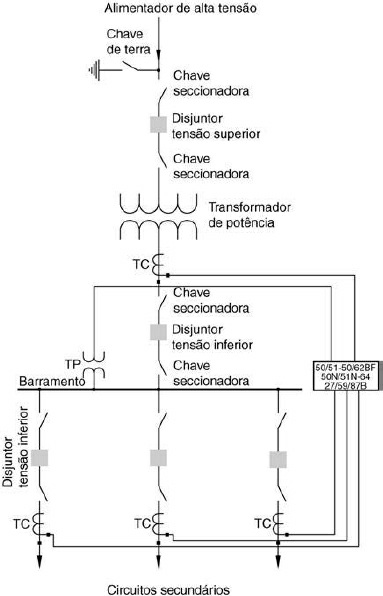
\includegraphics[scale = 0.9]{figuras/BarraSimplesPrimario.png}
    \\ Fonte: \cite{mamede2000protecao}
    \label{fig:BarraSimplesPrimario}
\end{figure}


\subsection{Barramento Simples com Barra de Transferência}

O barramento simples com barra de transferência, apresentado na figura \ref{fig:BarraTransferencia}, é utilizada em subestações de média e alta tensão. As manobras são realizadas sem que haja desligamentos e somente pode ser liberado um disjuntor de cada vez \cite{frontin2013equipamentos}. Esta configuração apresenta certa flexibilidade para manutenção e reparos, mas sua flexibilidade operativa é limitada, pois opera somente um barramento que limita a sua disponibilidade para ocorrência de falhas na barra e seccionadoras \cite{azevedo2015arranjos}. 

\begin{figure}[!htb] 
    \centering
    \caption{Proteção Barramento Simples com Barra de Transferência}
    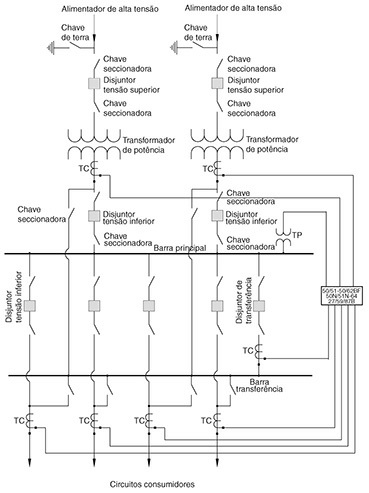
\includegraphics[scale = 1]{figuras/BarraTransferencia.png}
    \\ Fonte: \cite{mamede2000protecao}
    \label{fig:BarraTransferencia}
\end{figure}


\subsection{Barramento Simples Com Seccionamento de Barra}

O barramento simples com seccionamento de barra, apresentado na figura \ref{fig:BarraSeccionada}, é indicado para a condição de alimentação da subestação de dois ou mais circuitos de alta tensão e/ou quando há necessidade de se utilizar uma grande quantidade de circuitos de distribuição \cite{mamede2000protecao}. A flexibilidade para a manutenção das secções de barras tem uma sensível melhora, mantendo-se a subestação parcialmente em operação \cite{frontin2013equipamentos}.

\begin{figure}[!htb] 
    \centering
    \caption{Proteção Barramento Simples Com Seccionamento de Barra}
    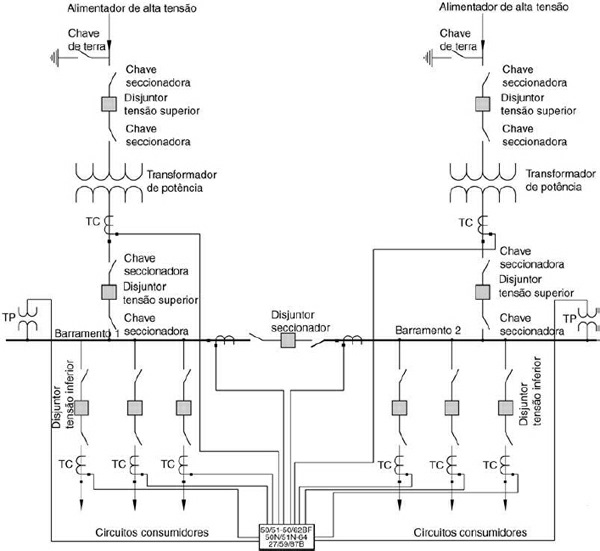
\includegraphics[scale = 0.7]{figuras/BarraSeccionada.png}
    \\ Fonte: \cite{mamede2000protecao}
    \label{fig:BarraSeccionada}
\end{figure}


\newpage

\subsection{Barramento Simples com Geração Auxiliar}

O barramento simples com geração auxiliar é semelhante ao arranjo anterior, com a diferença da fonte de geração auxiliar estar conectada à um dos barramentos (Ver Figura \ref{fig:BarraComGeracaoAuxiliar}). É indicado quando se necessita operar uma usina de geração termelétrica para funcionamento em emergência, na ponta de carga ou no controle da demanda por injeção de geração \cite{mamede2000protecao}.

\begin{figure}[!htb] 
    \centering
    \caption{Proteção Barramento Simples Com Geração Auxiliar}
    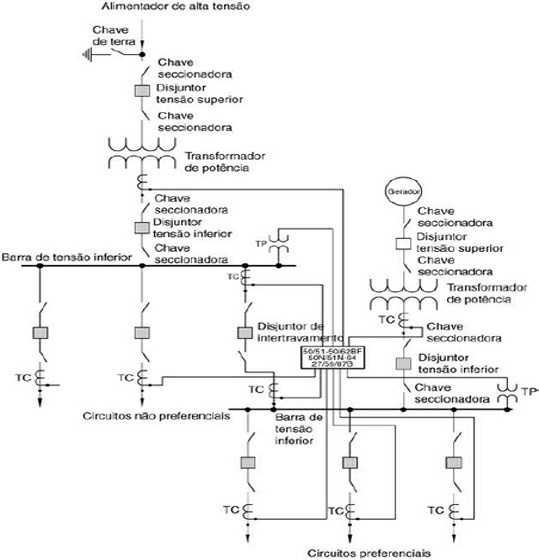
\includegraphics[scale = .75]{figuras/BarraComGeracaoAuxiliar.png}
    \\ Fonte: \cite{mamede2000protecao}
    \label{fig:BarraComGeracaoAuxiliar}
\end{figure}


\newpage

\subsection{Barramento Duplo a Quatro Chaves}

O barramento duplo a quatro chaves, apresentado na figura \ref{fig:BarraDupla4Chaves}, possui boa flexibilidade operativa e facilidades para a expansão, uma vez que se pode liberar temporariamente uma barra e não provocar desligamentos de circuitos do sistema \cite{holanda2016suel}. Nesta configuração, acrescenta-se uma chave de \textit{bypass} em cada \textit{bay}, de forma que todo disjuntor possa ser liberado para manutenção e reparos sem que seja necessário desligar o circuito correspondente \cite{frontin2013equipamentos}.

\begin{figure}[!htb] 
    \centering
    \caption{Proteção Barramento Duplo a Quatro Chaves}
    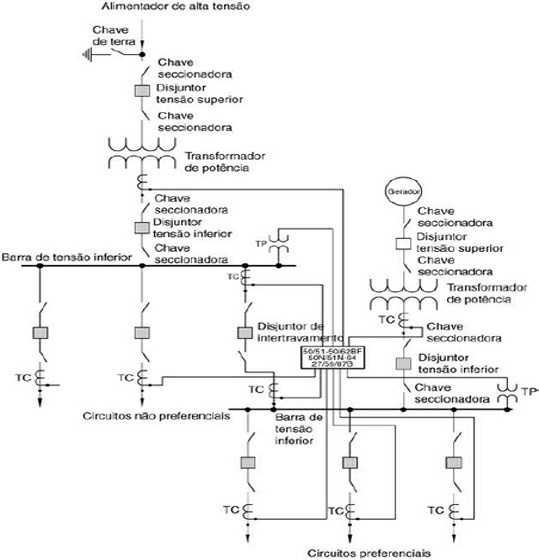
\includegraphics[scale = .8]{figuras/BarraComGeracaoAuxiliar.png}
    \\ Fonte: \cite{mamede2000protecao}
    \label{fig:BarraDupla4Chaves}
\end{figure}


\newpage

\subsection{Barramento Disjuntor Duplo}

O barramento disjuntor duplo, apresentado na figura \ref{fig:BarraDijuntorDuplo}, é caracterizado pela conexão dos circuitos de distribuição no ponto central entre
os dois barramentos \cite{mamede2000protecao}. Neste barramento a carga associada não é interrompida, caso ocorra um defeito em qualquer disjuntor dos circuitos secundários. 

\begin{figure}[!htb] 
    \centering
    \caption{Proteção Barramento Disjuntor Duplo}
    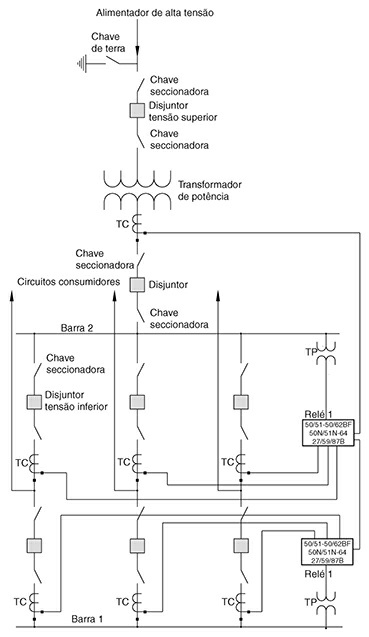
\includegraphics[scale = .8]{figuras/BarraDijuntorDuplo.png}
    \\ Fonte: \cite{mamede2000protecao}
    \label{fig:BarraDijuntorDuplo}
\end{figure}


\newpage

\subsection{Barramento Duplo e Disjuntor e Meio}

No barramento duplo e disjuntor e meio, apresentado na figura \ref{fig:BarraDijuntorMeio}, cada circuito pode ser alimentado por qualquer um dos barramentos por meio de um disjuntor central, que pode ser compartilhado por dois circuitos \cite{mamede2000protecao}.

\begin{figure}[!htb] 
    \centering
    \caption{Proteção Barramento Duplo e Disjuntor e Meio}
    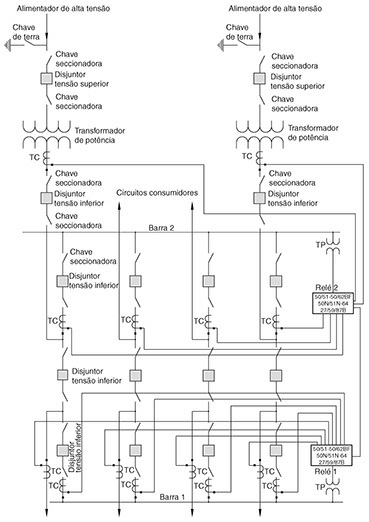
\includegraphics[scale = 1]{figuras/BarraDijuntorMeio.png}
    \\ Fonte: \cite{mamede2000protecao}
    \label{fig:BarraDijuntorMeio}
\end{figure}


\newpage

\subsection{Barramento em Anel}

Nesta configuração de barramento anel, embora econômica e flexível, tem o inconveniente de expor o sistema elétrico devido a falhas externas ao pátio em segundas contingências \cite{frontin2013equipamentos}. Segundo Holanda \citeyearpar{holanda2016suel}, apresenta a vantagem de dividir as cargas e controle do nível de falhas. Por outro lado, requer maior área de pátio em relação ao esquema de barra simples equivalente e quando um disjuntor estiver em manutenção, a abertura do outro
disjuntor não adjacente irá dividir o anel, podendo causar sérias perturbações no sistema.


\begin{figure}[H] 
    \centering
    \caption{Proteção Barramento Anel}
    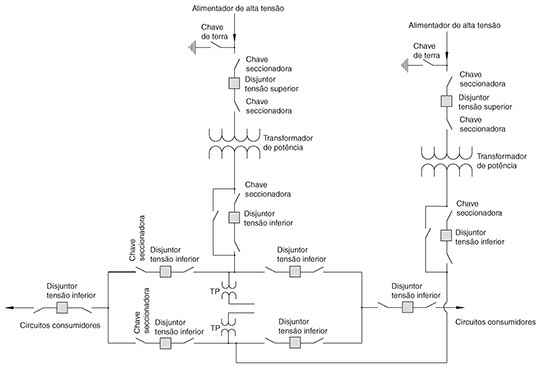
\includegraphics[scale = 1]{figuras/BarraAnel.png}
    \\ Fonte: \cite{mamede2000protecao}
    \label{fig:BarraAnel}
\end{figure}

%%======================================================================

\section{Tipos de Manobras}

\chapter{METODOLOGIA}

\section{Linguagem de Programação Python}

\subsection{Interface Gráfica}
\include{capitulos/5}
\include{capitulos/6}
\chapter{Conclusão}

Está é a conclusão do trabalho ....

\section{APRIMORAMENTO DO PROJETO E TRABALHOS FURUTOS}

\setlength{\baselineskip}{\baselineskip}

%%=============================================================================
%% Referências
%%=============================================================================
\bibliographystyle{abnt}
\bibliography{referencias/referencias}



%IMPORTANTE: Se precisar usar alguma seção ou subseção dentro dos apêndices ou
%anexos, utilizar o comando \tocless para não adicionar no Sumário
%Exemplos: 
% \tocless\section{Histórico}
%%=============================================================================
%% Apêndices
%%=============================================================================
%\appendix
%\chapter{Título do apêndice}
Este é o apêndice A

%IMPORTANTE: Se precisar usar alguma seção ou subseção dentro dos apêndices ou
%anexos, utilizar o comando \tocless para não adicionar no Sumário
%Exemplos: 
% \tocless\section{Histórico}
% \tocless\subsection{Detalhes}
\tocless\section{teste}
Este é um teste de seção dentro do apêndice


%\chapter{Título do apêndice Ex}
Esta é o apêndice B



%%=============================================================================
%% Anexos
%%=============================================================================
%\annex
%\chapter{Título do Anexo}
Este é o anexo A



\end{document}
